\section{Results}
\label{sec:results}

\begin{table*}[t]
  \centering
  \caption{Per-stratum citation $F_1$ across four settings. v2 main = DO-178C synthetic with local e5-small embeddings (4{,}440 runs); v3 main = same corpus with Azure text-embedding-3-small (4{,}440 runs); MuSiQue = 200-query Wikipedia stratified subset with Azure embedder (600 runs, vanilla / agentic-graph / graphrag only); 2Wiki = 200-query 2WikiMultihopQA subset at three seeds (1{,}200 runs, vanilla / graphrag only). Bold marks the per-(setting, stratum) maximum. The stratum-conditional pattern is the same on all four: vanilla is competitive at 1-hop and loses as hop distance grows.}
  \label{tab:dominance}
  \footnotesize\setlength{\tabcolsep}{3pt}
  \resizebox{\textwidth}{!}{%
  \begin{tabular}{l ccc | ccc | ccc | ccc}
    \toprule
     & \multicolumn{3}{c|}{v2 main (local)} & \multicolumn{3}{c|}{v3 main (Azure)} & \multicolumn{3}{c|}{MuSiQue (Azure)} & \multicolumn{3}{c}{2Wiki (Azure)} \\
    System & 1h & 2h & 3+h & 1h & 2h & 3+h & 1h & 2h & 3+h & 1h & 2h & 3+h \\
    \midrule
    vanilla & \textbf{.757} & .712 & .089 & \textbf{.756} & .689 & .195 & .742 & .415 & .277 & \textbf{.990} & .778 & .678 \\
    agentic & .541 & .414 & .175 & .533 & .430 & .203 & --- & --- & --- & --- & --- & --- \\
    agentic-graph & .566 & .415 & \textbf{.219} & .547 & .421 & .251 & .457 & .296 & .249 & --- & --- & --- \\
    graphrag & .751 & \textbf{.720} & .172 & .745 & \textbf{.707} & .253 & \textbf{.841} & \textbf{.632} & \textbf{.463} & .969 & \textbf{.946} & \textbf{.938} \\
    adaptive & .630 & .499 & .181 & .651 & .492 & \textbf{.254} & --- & --- & --- & --- & --- & --- \\
    \bottomrule
  \end{tabular}}
\end{table*}


\begin{figure}[t!]
  \centering
  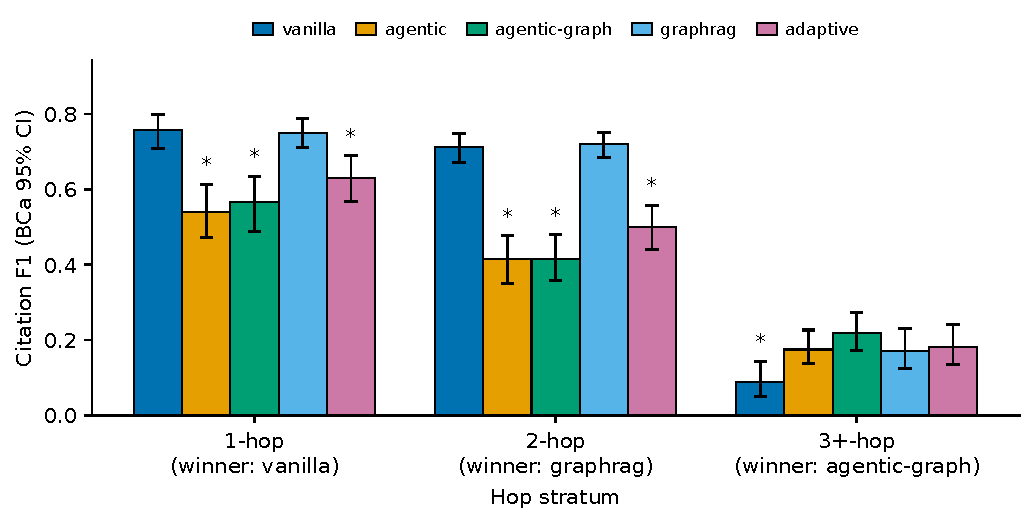
\includegraphics[width=0.55\textwidth]{figures/fig1_per_stratum_f1.pdf}
  \caption{Per-stratum citation $F_1$ on the v2 main matrix (DO-178C,
    local e5-small embedder): five pipelines with BCa 95\% CIs;
    \mbox{$*$} marks pipelines significantly different from the
    per-stratum winner (Holm-Wilcoxon $p{<}0.05$,
    $|\delta|{\geq}0.147$).}
  \Description{Grouped bar chart of per-stratum citation F1 for five
    RAG pipelines (vanilla, agentic, agentic-graph, graphrag, adaptive)
    on the DO-178C v2 main matrix, broken down by 1-hop, 2-hop, and
    3+-hop strata, with error bars and asterisks marking pipelines
    significantly different from the per-stratum winner.}
  \label{fig:perstratum}
\end{figure}

\subsection{C1: Winners are Corpus-Conditional, Embedder- and Seed-Robust}
\label{sec:c1}
Table~\ref{tab:dominance} reports per-stratum $F_1$ across four settings.
On DO-178C, vanilla and GraphRAG are statistically tied on 1-hop and
2-hop (Wilcoxon $p{=}0.12/0.65$ local, negligible $\delta$), the
agentic loop costs 0.19--0.30 $F_1$ on those strata, and on 3+-hop the
ordering inverts: vanilla drops to last and the graph-aided pipelines
lead (local: agentic-graph 0.219 vs.\ vanilla 0.089, Holm
$p{<}10^{-6}$; under Azure the ordering holds but no 3+-hop pair passes
the joint criterion). A third embedder from a third vendor (bge-m3)
reproduces it (Table~\ref{tab:embedders}): vanilla is last at 3+-hop
under all three, and under bge-m3 both graph arms beat it ($+0.100$,
$+0.091$; Holm $p{=}2.1{\times}10^{-4}$, $1.4{\times}10^{-3}$) while
1--2-hop contrasts stay negligible. On MuSiQue GraphRAG wins every
stratum ($F_1{=}0.841/0.632/0.463$; $p{\leq}5.1{\times}10^{-4}$,
$\delta{=}0.27$--$0.43$). Because MuSiQue's \textit{REFERENCES} edges
connect only gold paragraphs, we re-ran GraphRAG with
consecutive-distractor edges added: it loses only $0.02/0.05/0.09$ $F_1$
and still beats vanilla everywhere ($p{\leq}0.014$). On 2WikiMultihopQA
the two are tied at 1-hop ($p{=}0.15$) and GraphRAG wins 2-hop and
3+-hop by widening margins ($+0.168$, $+0.260$; $\delta{=}0.48$, $0.87$)
-- the same crossover on a graph we did not design. Seed variance is
small against these effects: per-pipeline mean $F_1$ moves by at most
$0.031$ across seeds, every significant ordering holds in each seed
separately, and the only rank swaps are within the vanilla--GraphRAG
pairs we report as tied.

\begin{table}[t]
  \centering
  \caption{Per-stratum citation $F_1$ on DO-178C under three independent embedders (384d Microsoft, 1536d OpenAI, 1024d BAAI). The stratum-conditional ordering is stable: vanilla ties GraphRAG on 1--2-hop and is \emph{last} at 3+-hop in all three, where a graph-aided pipeline leads.}
  \label{tab:embedders}
  \small
  \setlength{\tabcolsep}{4pt}
    \begin{tabular}{l rrr rrr rrr}
    \toprule
    & \multicolumn{3}{c}{e5-small (384d)} & \multicolumn{3}{c}{3-small (1536d)} & \multicolumn{3}{c}{bge-m3 (1024d)} \\
    \cmidrule(lr){2-4}\cmidrule(lr){5-7}\cmidrule(lr){8-10}
    System & 1h & 2h & 3+h & 1h & 2h & 3+h & 1h & 2h & 3+h \\
    \midrule
    vanilla       & \textbf{.757} & .712 & .089 & \textbf{.756} & .689 & .195 & \textbf{.769} & .691 & .114 \\
    agentic       & .541 & .414 & .175 & .533 & .430 & .203 & .548 & .404 & .156 \\
    agentic-graph & .566 & .415 & \textbf{.219} & .547 & .421 & .251 & .546 & .431 & .206 \\
    graphrag      & .751 & \textbf{.720} & .172 & .745 & \textbf{.707} & .253 & .742 & \textbf{.728} & \textbf{.214} \\
    adaptive      & .630 & .499 & .181 & .651 & .492 & \textbf{.254} & .672 & .478 & .202 \\
    \bottomrule
  \end{tabular}
\end{table}


\begin{table}[t]
  \centering
  \caption{GraphRAG floods the context and the synthesizer filters it (C2), across every setting we ran: three embedders, three corpora, and two traversals. The walk fills 11--15 slots at low precision; the answer cites 2.5--5.0 IDs at 3--4$\times$ that precision. The ranking inverts with the measurement point in all six.}
  \label{tab:pathology}
  \small
  \setlength{\tabcolsep}{4pt}
  \begin{tabular}{l rr rr r}
    \toprule
    & \multicolumn{2}{c}{\textit{retrieved context}} & \multicolumn{2}{c}{\textit{answer citations}} & \\
    \cmidrule(lr){2-3}\cmidrule(lr){4-5}
    Setting & slots & prec. & IDs & prec. & gain \\
    \midrule
    DO-178C, e5-small     & 14.9 & 0.120 & 4.9 & 0.480 & 4.0$\times$ \\
    DO-178C, 3-small      & 14.9 & 0.129 & 5.0 & 0.493 & 3.8$\times$ \\
    DO-178C, bge-m3       & 14.8 & 0.121 & 4.7 & 0.490 & 4.1$\times$ \\
    DO-178C, PPR walk     & 14.9 & 0.131 & 4.9 & 0.509 & 3.9$\times$ \\
    MuSiQue               & 11.2 & 0.227 & 3.4 & 0.654 & 2.9$\times$ \\
    2WikiMultihopQA       & 11.4 & 0.230 & 2.5 & 0.975 & 4.2$\times$ \\
    \bottomrule
  \end{tabular}
\end{table}


\begin{figure}[t!]
  \centering
  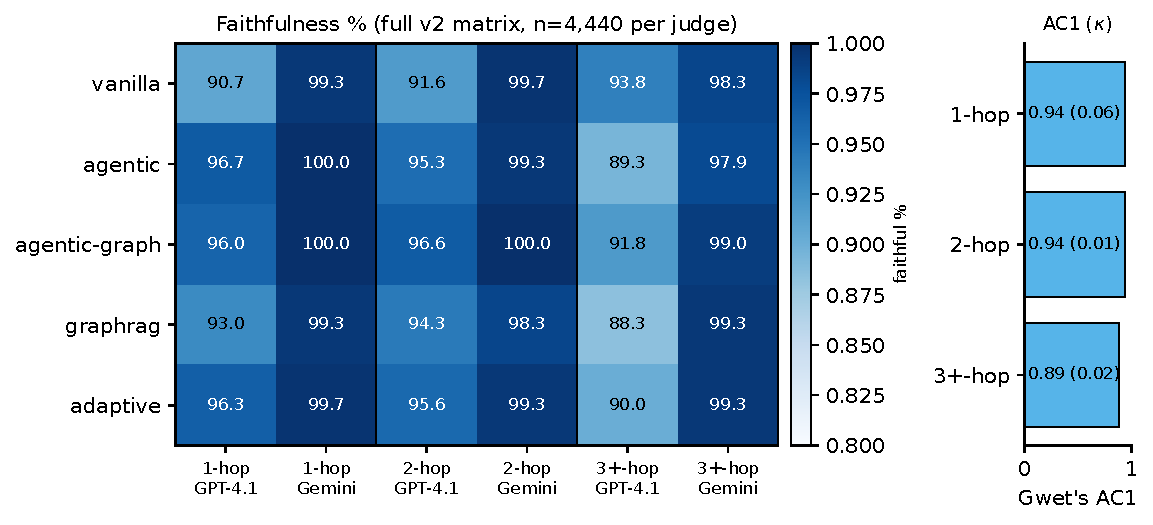
\includegraphics[width=0.8\textwidth]{figures/fig2_faithfulness_heatmap.pdf}
  \caption{Faithfulness on the full v2 main matrix (DO-178C, e5-small;
    4{,}440 rows, $\approx$300 per cell), judged by GPT-4.1 and Gemini
    3.7-flash on identical rows. \textit{Left}: under GPT-4.1 every
    expanding pipeline loses 4--7\,pp from 1-hop to 3+-hop while vanilla,
    which expands nothing, does not decline (C3); Gemini compresses every
    cell against the ceiling. \textit{Right}: per-stratum Gwet's AC1 with
    Cohen's $\kappa$ in parentheses -- 0.89--0.94 against
    $\kappa{\leq}0.06$ on the same verdicts, the prevalence paradox of
    C4. Colour scale starts at 80\%.}
  \Description{Heatmap of faithfulness percentages for five RAG
    pipelines (rows: vanilla, agentic, agentic-graph, graphrag,
    adaptive) across three hop strata times two judges (columns:
    1-hop GPT-4.1, 1-hop Gemini, 2-hop GPT-4.1, 2-hop Gemini,
    3+-hop GPT-4.1, 3+-hop Gemini) on the full v2 main matrix. Under
    GPT-4.1 the expanding pipelines lighten toward 3+-hop while vanilla
    does not; Gemini cells are uniformly near 99\%. A side panel shows
    per-stratum Gwet AC1 bars annotated with Cohen's kappa.}
  \label{fig:faithheatmap}
\end{figure}

\subsection{C2: The Walk Floods the Context, the Synthesizer Filters It}
\label{sec:c2}
\noindent Table~\ref{tab:pathology} reports the same measurement in
six settings: three embedders, three corpora, and two traversals.
GraphRAG's walk fills 11--15 context slots at context precision
0.12--0.23 -- four to five of every six retrieved chunks are off-gold.
The synthesizer then cites only 2.5--5.0 IDs per answer, at citation
precision 0.48--0.98: a 2.9--4.2$\times$ precision enrichment over its
own context, in every setting. GraphRAG's $F_1$ edge is therefore a
\emph{recall} effect: the walk surfaces gold chunks dense retrieval
misses, and the synthesizer declines to cite most of the noise that
rides along. Evaluations that score the retrieved set as the
attribution set -- as some GraphRAG comparisons do -- measure the
flooding and miss the filtering, and invert the ranking: by context
precision GraphRAG sits below the vanilla baseline in every setting
($0.12$--$0.23$ against $0.27$--$0.37$), while by answer-citation $F_1$
it is the highest-scoring pipeline in every setting ($0.551$, $0.571$,
$0.565$, $0.585$, $0.646$, $0.951$ in the row order of
Table~\ref{tab:pathology}). The two measurements do not merely differ in
magnitude; they disagree on the sign of the comparison that the
architecture debate turns on.

Two controls show the split is not an artifact of our own design
choices. First, \emph{traversal}: replacing the bounded 2-hop walk with
personalized PageRank over the same graph -- unbounded in radius and
ranked by random-walk mass rather than hop distance, with embedder,
seeds and context cap held fixed -- changes almost nothing (context
precision $0.131$ vs.\ $0.129$, and $0.131$ for the 2-hop walk rebuilt
on the same file-backed graph, \S\ref{sec:experiments}; enrichment $3.9\times$ vs.\
$3.8\times$; citation $F_1$ $+0.016$ at Cliff's $\delta{=}0.036$, which
our joint criterion rejects as negligible). Second, \emph{mitigation}:
neither obvious fix helps. Reranking the walked neighbours by query
similarity and keeping the top five leaves everything where it was
(context precision $0.227{\to}0.232$, citation $F_1$ $+0.010$,
$p{=}0.34$), while tightening the traversal budget actively hurts
(walk $30{\to}10$, context $15{\to}8$: citation $F_1$ $-0.126$,
$p{=}2.6{\times}10^{-11}$, and context precision \emph{falls} to
$0.194$). This is what C2 predicts: the synthesizer already performs
the filtering, so filtering again upstream is redundant, and cutting
the budget only removes the recall the advantage rests on.

\subsection{C3: The Decline Follows Context Expansion, Not the Corpus}
\label{sec:c3}
Judged on 300-row subsets, the faithfulness decline looks
\emph{corpus-conditional}: present on DO-178C, absent on Wikipedia
chains. That reading does not survive adequate power. The MuSiQue arm
had 67 rows per stratum; its 1-hop to 3+-hop drop ($9.2$\,pp) was larger
than the $4.7$\,pp that reaches significance on DO-178C, but detecting
it at 80\% power needs about 210 rows per cell. At three seeds
($n{=}600$) the decline is significant under both judges:
$0.930/0.876/0.823$ under GPT-4.1 ($p{=}1.1{\times}10^{-3}$) and
$0.955/0.945/0.869$ under Gemini ($p{=}1.2{\times}10^{-3}$).
2WikiMultihopQA, judged in full ($n{=}1{,}200$), declines as well
($p{=}5.0{\times}10^{-2}$ and $4.8{\times}10^{-6}$), so the decline
replicates on three corpora under two vendors.

What separates pipelines is whether they expand the context at all.
Vanilla, the only pipeline that retrieves a fixed top-5 and expands
nothing, shows no significant 1-hop to 3+-hop drop under GPT-4.1:
${-}1.5$\,pp on DO-178C ($n{=}2{,}072$, per-embedder $p{=}0.16$,
$0.99$, $0.76$) and $+1.1$\,pp on 2Wiki ($p{=}0.66$), against $6.3$ and
$6.7$\,pp for the four expanding pipelines. A logistic fit of
faithfulness on hop, an expansion indicator and their interaction makes
this a single test: the interaction is negative and significant on the
pooled DO-178C matrix ($b{=}{-}0.599$, $p{=}1.0{\times}10^{-7}$,
$n{=}10{,}360$) and negative but not significant on 2Wiki
($b{=}{-}0.286$, $p{=}0.27$), whose arm is a twentieth the size.
Under Gemini the ordering holds but the test does not resolve: near the
ceiling the baseline itself acquires a slope ($b{=}{-}0.729$,
$p{=}0.012$) and the interaction is not separable from it ($p{=}0.11$),
though expanding arms still drop further than vanilla ($2.8$ vs.\
$1.5$\,pp on DO-178C, $12.7$ vs.\ $7.7$\,pp on 2Wiki) -- a lenient judge
preserves the ranking and loses the resolution (C4). We do not claim
every expanding pipeline declines in every cell: GraphRAG is marginal
under bge-m3 ($p{=}0.065$), and the agentic arms decline in four of six
embedder--pipeline combinations. The GPT-5.4 leg has not been re-run at
this power.

\begin{table}[t]
  \centering
  \caption{Judge stability. \textit{Top}: same judge, frozen input --- the answer and context strings are identical and only the judging date differs, so the fall from 0.76 to 0.14 isolates drift from any retrieval effect. \textit{Middle}: same judge, input changed by embedder swap. \textit{Bottom}: cross-vendor agreement on identical rows. Which judge is stricter depends on the corpus --- Gemini is markedly more lenient on DO-178C, indistinguishable on the capped MuSiQue arm, and stricter on 2Wiki. Raw agreement and AC1 move together across the eight settings while $\kappa$ swings by a factor of fifteen, ordered by distance from the ceiling.}
  \label{tab:judges}
  \small
  \setlength{\tabcolsep}{4pt}
    \begin{tabular}{l rrrr}
    \toprule
    \multicolumn{5}{l}{\textit{Same judge, frozen input (answer + context identical)}} \\
    \midrule
    GPT-5.4, re-judged same day & \multicolumn{4}{r}{$\kappa = 0.764$, raw agr.\ 0.88} \\
    GPT-5.4, re-judged 11 wk later & \multicolumn{4}{r}{$\kappa = 0.138$, raw agr.\ 0.56} \\
    GPT-4.1, re-judged 11 wk later & \multicolumn{4}{r}{$\kappa = -0.05\,/\,-0.00$ (v2/v3), raw agr.\ 0.48\,/\,0.51} \\
    GPT-4.1, full matrix vs.\ May & \multicolumn{4}{r}{$\kappa = -0.046$, raw agr.\ 0.48, $+43$\,pp} \\
    \midrule
    \multicolumn{5}{l}{\textit{Same judge, input changed by embedder swap}} \\
    \midrule
    GPT-5.4 (v2 vs v3) & \multicolumn{4}{r}{$\kappa = 0.137$, raw agr.\ 0.59} \\
    GPT-4.1 (v2 vs v3) & \multicolumn{4}{r}{$\kappa = 0.480$, raw agr.\ 0.74} \\
    \midrule
    \multicolumn{5}{l}{\textit{Cross-vendor, same rows, one judging window (Gemini 3.7-flash $\times$ GPT-4.1)}} \\
    \midrule
    \textit{Setting} & raw & $\kappa$ & AC1 & faithful (G\,/\,4.1) \\
    \midrule
    DO-178C e5-small ($n{=}4{,}440$) & 0.929 & 0.029 & 0.923 & 0.993 / 0.933 \\
    DO-178C 3-small ($n{=}4{,}440$)  & 0.913 & 0.125 & 0.903 & 0.980 / 0.917 \\
    DO-178C bge-m3 ($n{=}1{,}480$)   & 0.939 & 0.047 & 0.935 & 0.991 / 0.945 \\
    DO-178C PPR walk ($n{=}296$)     & 0.926 & 0.058 & 0.919 & 0.983 / 0.936 \\
    MuSiQue, 3 seeds ($n{=}600$)     & 0.850 & 0.172 & 0.817 & 0.923 / 0.877 \\
    MuSiQue rerank ($n{=}200$)       & 0.820 & 0.171 & 0.772 & 0.935 / 0.825 \\
    MuSiQue budget cap ($n{=}200$)   & 0.875 & 0.419 & 0.841 & 0.875 / 0.880 \\
    2WikiMultihopQA ($n{=}1{,}200$)  & 0.899 & 0.435 & 0.877 & 0.888 / 0.914 \\
    \bottomrule
  \end{tabular}
\end{table}

\subsection{C4: Judges Are Unstable on Frozen Inputs and on Changed Ones}
\label{sec:c4}
\looseness=-1
Table~\ref{tab:judges} separates judge instability measured on
\emph{frozen} inputs, where no retrieval is re-run, from instability
under a changed retrieval state.
\noindent\textit{Frozen inputs.} Re-judging the identical 300 stored
(answer, context) pairs gives GPT-5.4 $\kappa{=}0.76$ (raw agreement
0.88) on the same day but only $\kappa{=}0.14$ (0.56) eleven weeks
later, a $+15$\,pp leniency shift that rejects a stationary judge
(binomial $p{<}10^{-44}$). GPT-4.1 on the same tuples falls to chance
agreement with its own earlier verdicts ($\kappa{=}{-}0.05/{-}0.00$),
$+41$\,pp more lenient. With inputs fixed, this is judge drift alone.
\noindent\textit{Changed retrieval state.} After an embedder swap,
which changes contexts and answers on 94\% of tuples, GPT-5.4 flips 41\%
of verdicts ($\kappa{=}0.137$) and GPT-4.1 26\% ($\kappa{=}0.48$): the
judge more stable under embedder swap is the less stable across time.
\noindent\textit{Across vendors.} On identical rows, Gemini 3.7-flash is
far more lenient than GPT-4.1 on all four DO-178C settings (0.98--0.99
vs.\ 0.92--0.95 faithful; McNemar $p{<}10^{-9}$), indistinguishable on
the budget-capped MuSiQue arm ($0.875$ vs.\ $0.880$, $p{=}1.00$), and
\emph{stricter} on 2WikiMultihopQA ($0.888$ vs.\ $0.914$,
$p{=}6.2{\times}10^{-3}$). Strictness is a property of the judge--corpus
pair and cannot be calibrated once and reused. The same eight settings
expose the prevalence paradox~\cite{feinstein1990} within one judge
pair: raw agreement moves only from 0.82 to 0.94 and Gwet's AC1 tracks
it (0.77--0.94), but $\kappa$ swings from $0.03$ to $0.44$, ordered
almost exactly by distance from the ceiling. On 2Wiki the pair agrees
\emph{less} often than on DO-178C (0.899 vs.\ 0.93) yet appears fifteen
times more reliable by $\kappa$ ($0.435$ vs.\ $0.029$). Leniency and
\emph{trend} nonetheless come apart: near the ceiling, Gemini still
reproduces the hop-wise decline on both DO-178C matrices
($p{=}4.3{\times}10^{-3}$, $p{<}10^{-16}$) and on both Wikipedia corpora.
The ordering a judge induces replicates across vendors; its strictness
does not.

\noindent\textit{Between judges, and why we re-judged everything.}
Inter-judge $\kappa$ halves under embedder swap on identical tuples
(0.30 $\to$ 0.17; McNemar $p{<}0.001$), and on the 300-row MuSiQue
batch GPT-5.4 and GPT-4.1 agreed at chance (raw agreement 0.48, AC1
0.08 -- genuine disagreement, not a prevalence artifact). Verdicts this
unstable cannot carry a cross-corpus claim, which is why the full matrix
was re-judged inside a single window (\S\ref{sec:c3}); no faithfulness
comparison we report spans judging dates.
